\documentclass[aspectratio=169]{beamer}
\usepackage{../theme/cs2theme}
\usepackage{../theme/cs2commands}
\usepackage{graphicx}
\setcsweek{Week 3}
\title{Found Your World}
\subtitle{A verified path from model limits to a World Bible v0.1}
\author{Computer Science II \textbullet\ Dr. Jeremy P. Evert}
\date{August 31, 2026}
\graphicspath{{img/}}
\begin{document}
\begin{frame}[plain]\titlepage\end{frame}
\begin{destinationframe}{Today's destination}
  \begin{itemize}
    \item Separate “it runs” from “it runs usefully.”
    \item Match a model and a bounded task to available hardware.
    \item Verify output with a diff and an independent test.
    \item Draft a fictional world seed: World Bible v0.1.
  \end{itemize}
\end{destinationframe}
\begin{frame}{The reframe}
  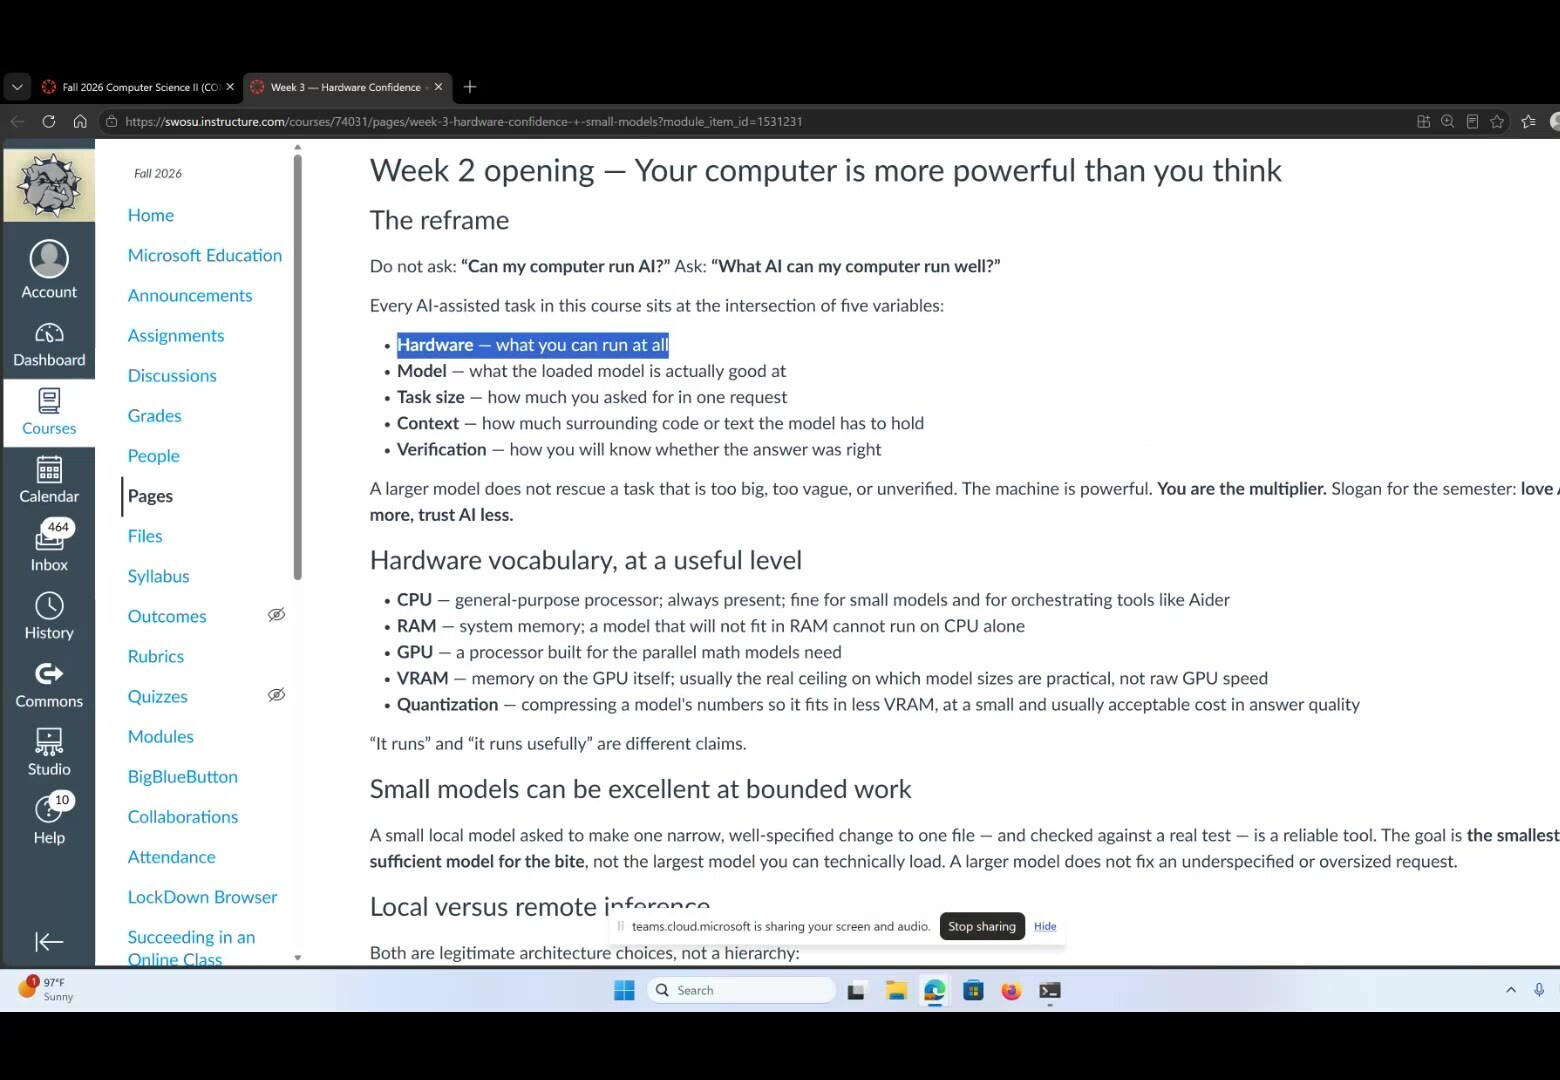
\includegraphics[width=.78\textwidth,height=.62\textheight,keepaspectratio]{reframe}
  \vfill\centering\large It runs \emph{versus} it runs usefully.
\end{frame}
\begin{frame}{The bite ladder}
  \begin{enumerate}
    \item Give the model one small, bounded task.
    \item Inspect the diff — read every changed line.
    \item Run an independent test, not the model's claim.
    \item If it holds, take one rung up: task or context.
    \item If it breaks, you found a boundary; back off a rung.
  \end{enumerate}
  \vfill\centering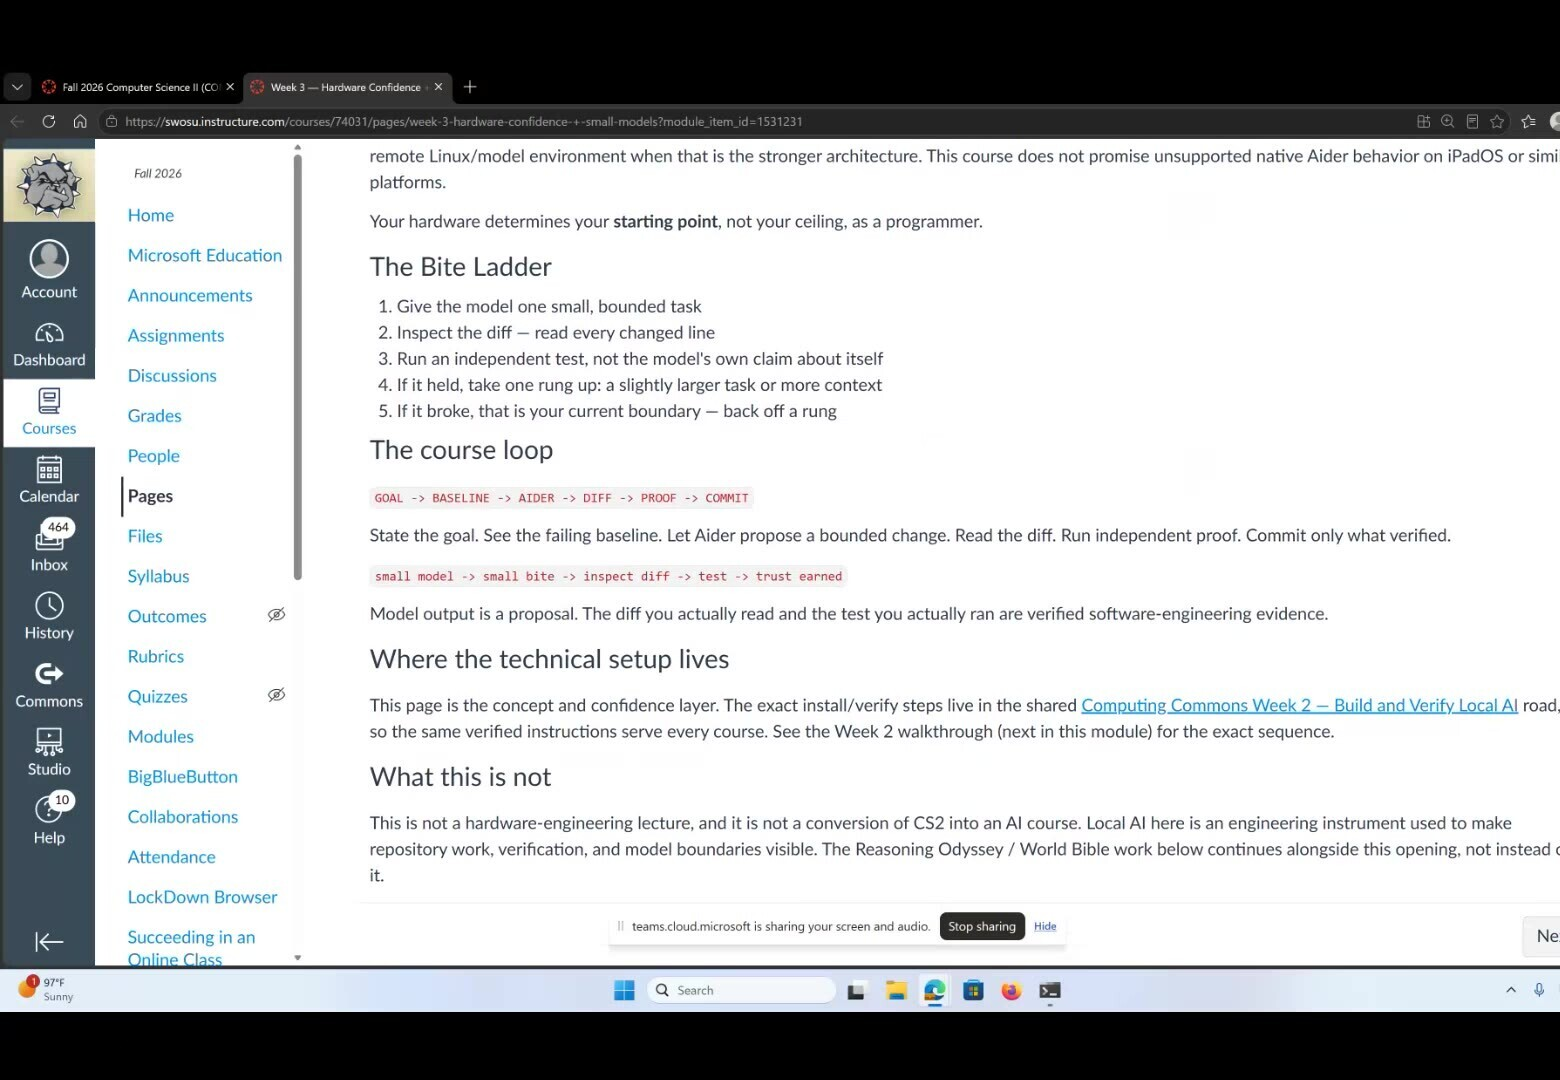
\includegraphics[width=.70\textwidth,height=.34\textheight,keepaspectratio]{add_test}
\end{frame}
\begin{frame}{See what models you actually have}
  \begin{columns}[T]
    \column{.48\textwidth}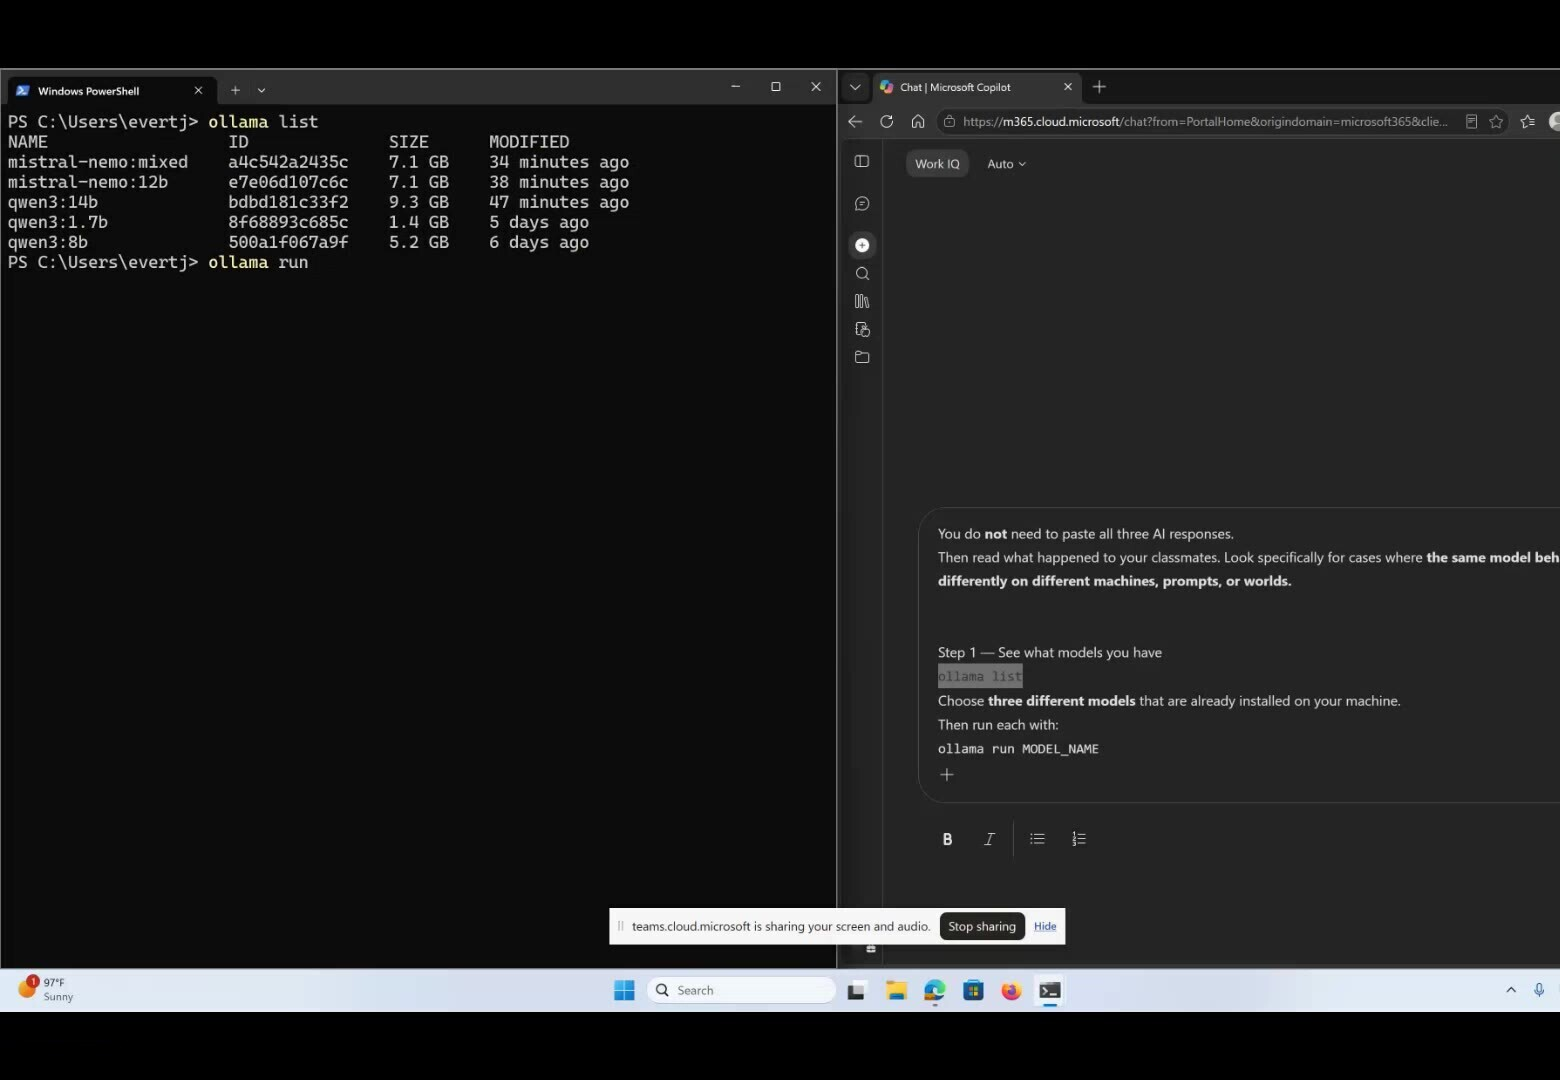
\includegraphics[width=\textwidth]{model_list}
    \column{.48\textwidth}\begin{itemize}\item `ollama list` inventories installed models.\item Size changes the fit, speed, and boundary.\item Choose the smallest sufficient model for the bite.\end{itemize}
  \end{columns}
\end{frame}
\begin{frame}{A World Bible is a design seed}
  \begin{columns}[T]
    \column{.48\textwidth}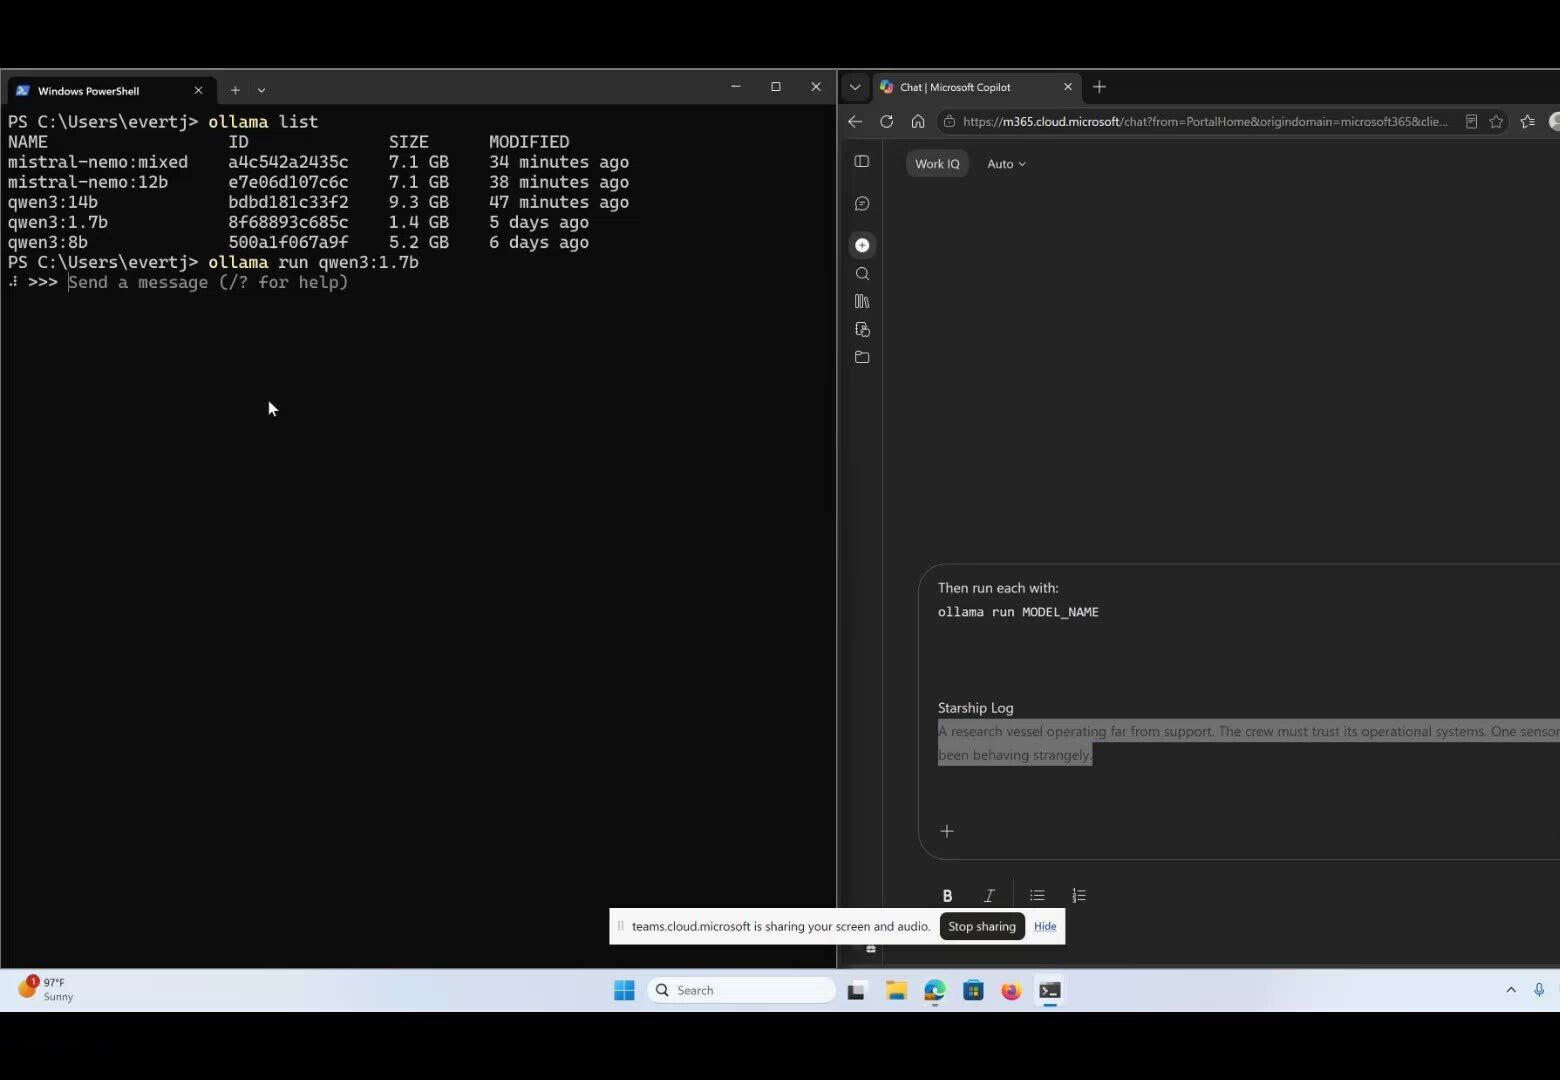
\includegraphics[width=\textwidth]{world_prompt}
    \column{.48\textwidth}\begin{itemize}\item Choose Frontier Settlement, Investigation Bureau, Starship Log, or Small Business.\item Write a premise, cast, one flow, questions, unknowns, and object predictions.\item You are allowed to be wrong.\end{itemize}
  \end{columns}
\end{frame}
\begin{frame}{Mismatch is evidence}
  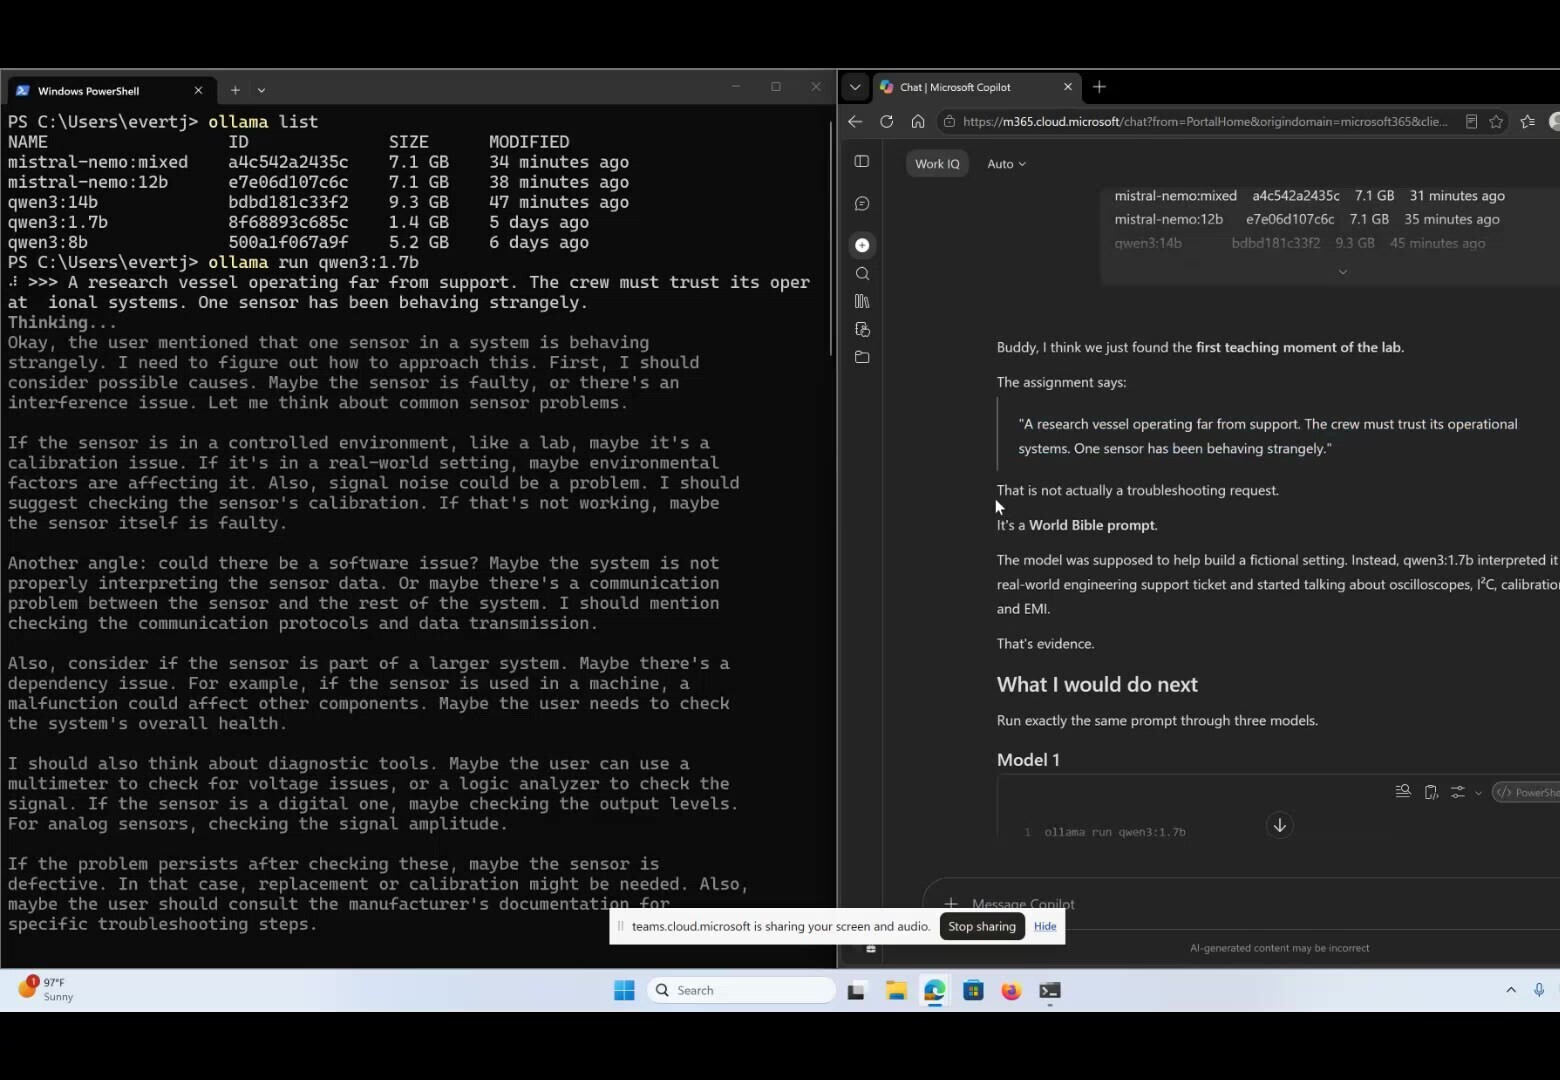
\includegraphics[width=.78\textwidth,height=.62\textheight,keepaspectratio]{wrong_fit}
  \vfill\centering The fictional prompt became an engineering ticket. Diagnose the mismatch.
\end{frame}
\begin{frame}{Fit is a memory question}
  \begin{columns}[T]
    \column{.48\textwidth}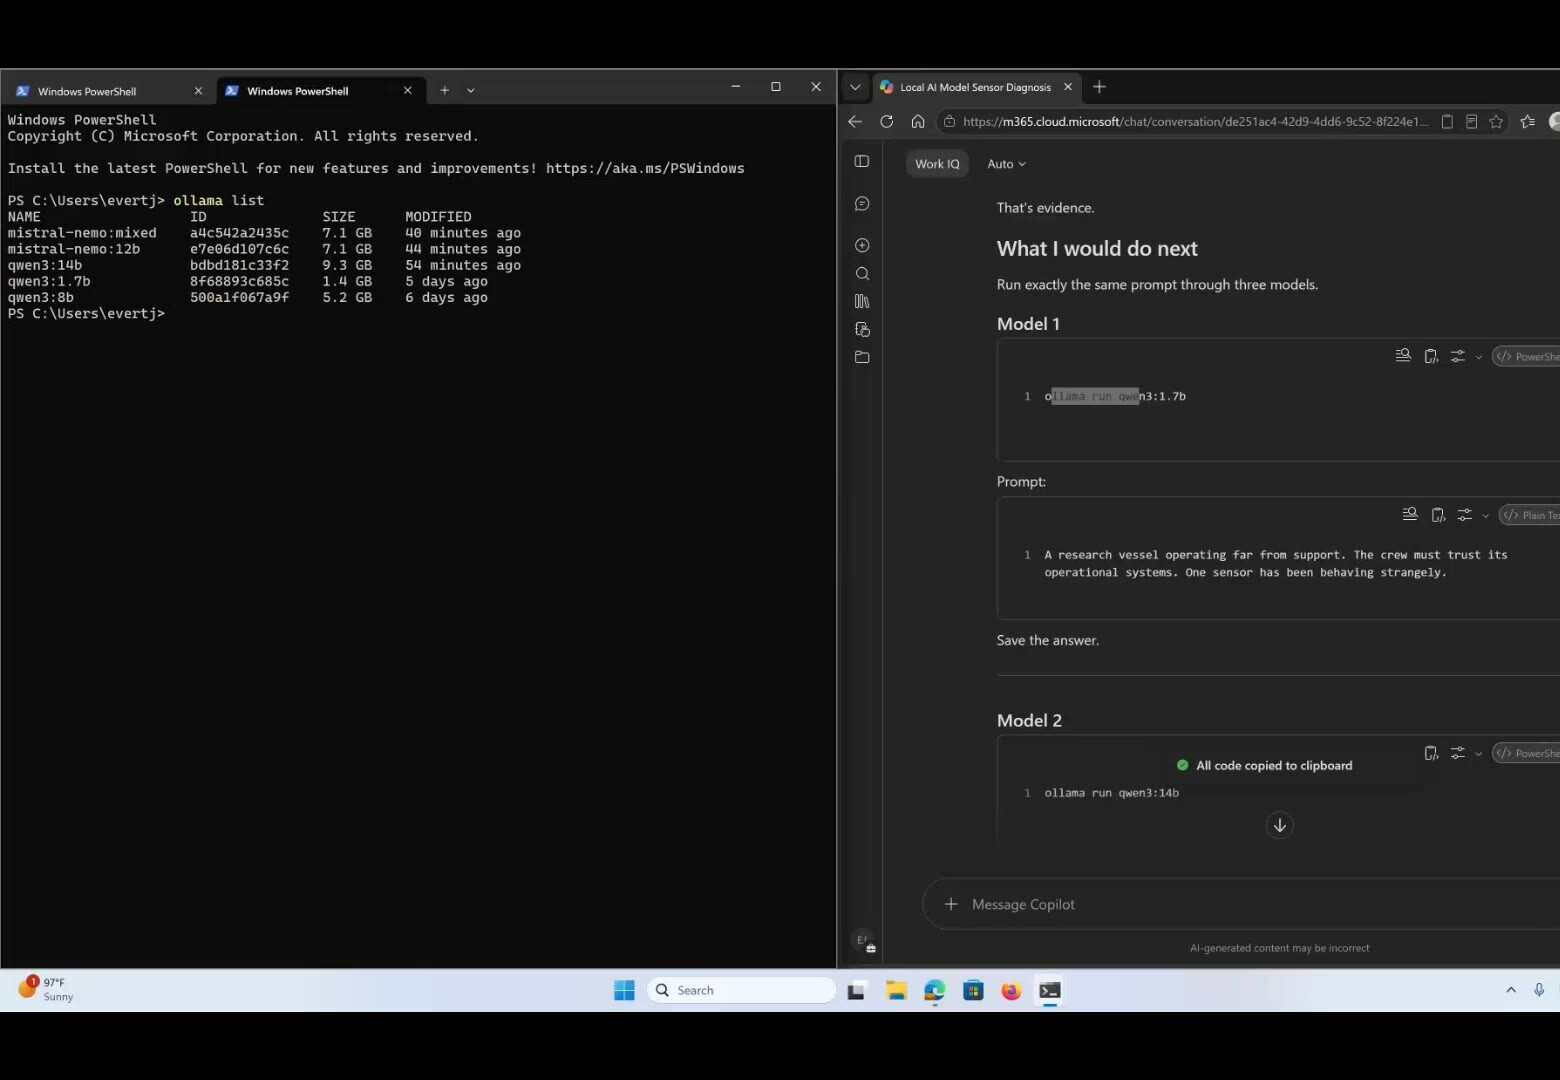
\includegraphics[width=\textwidth]{model_sizes}
    \column{.48\textwidth}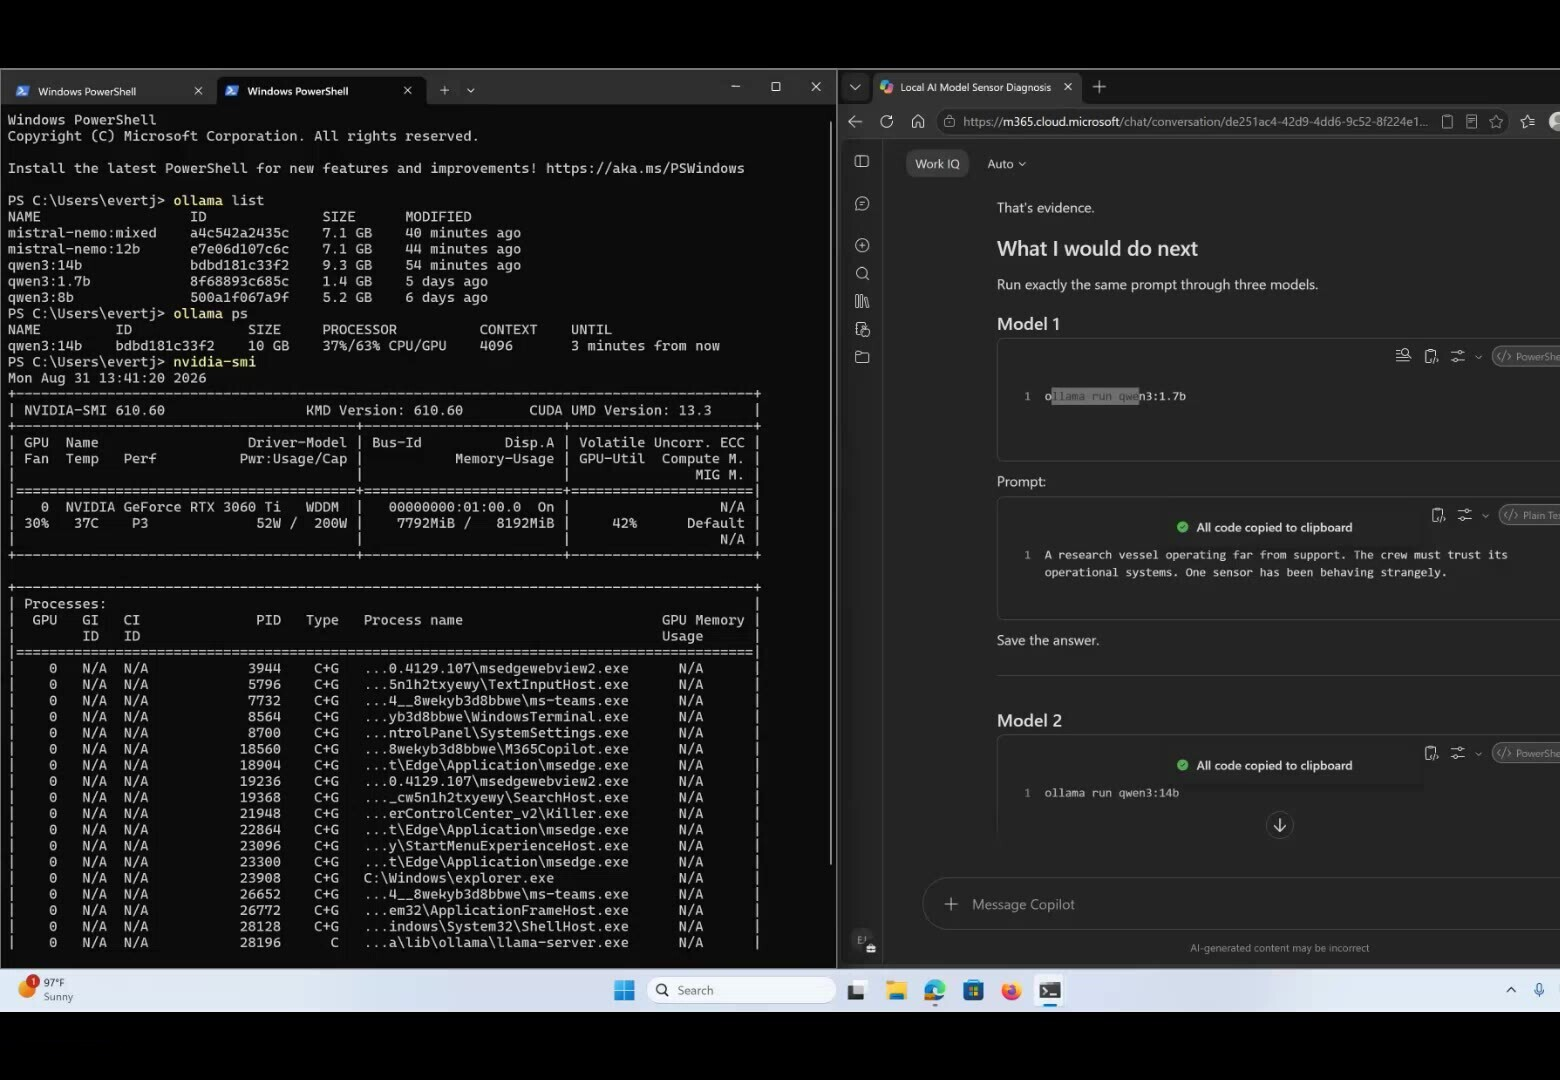
\includegraphics[width=\textwidth]{gpu_vram}
  \end{columns}
\end{frame}
\begin{frame}{GPU-only is not always the answer}
  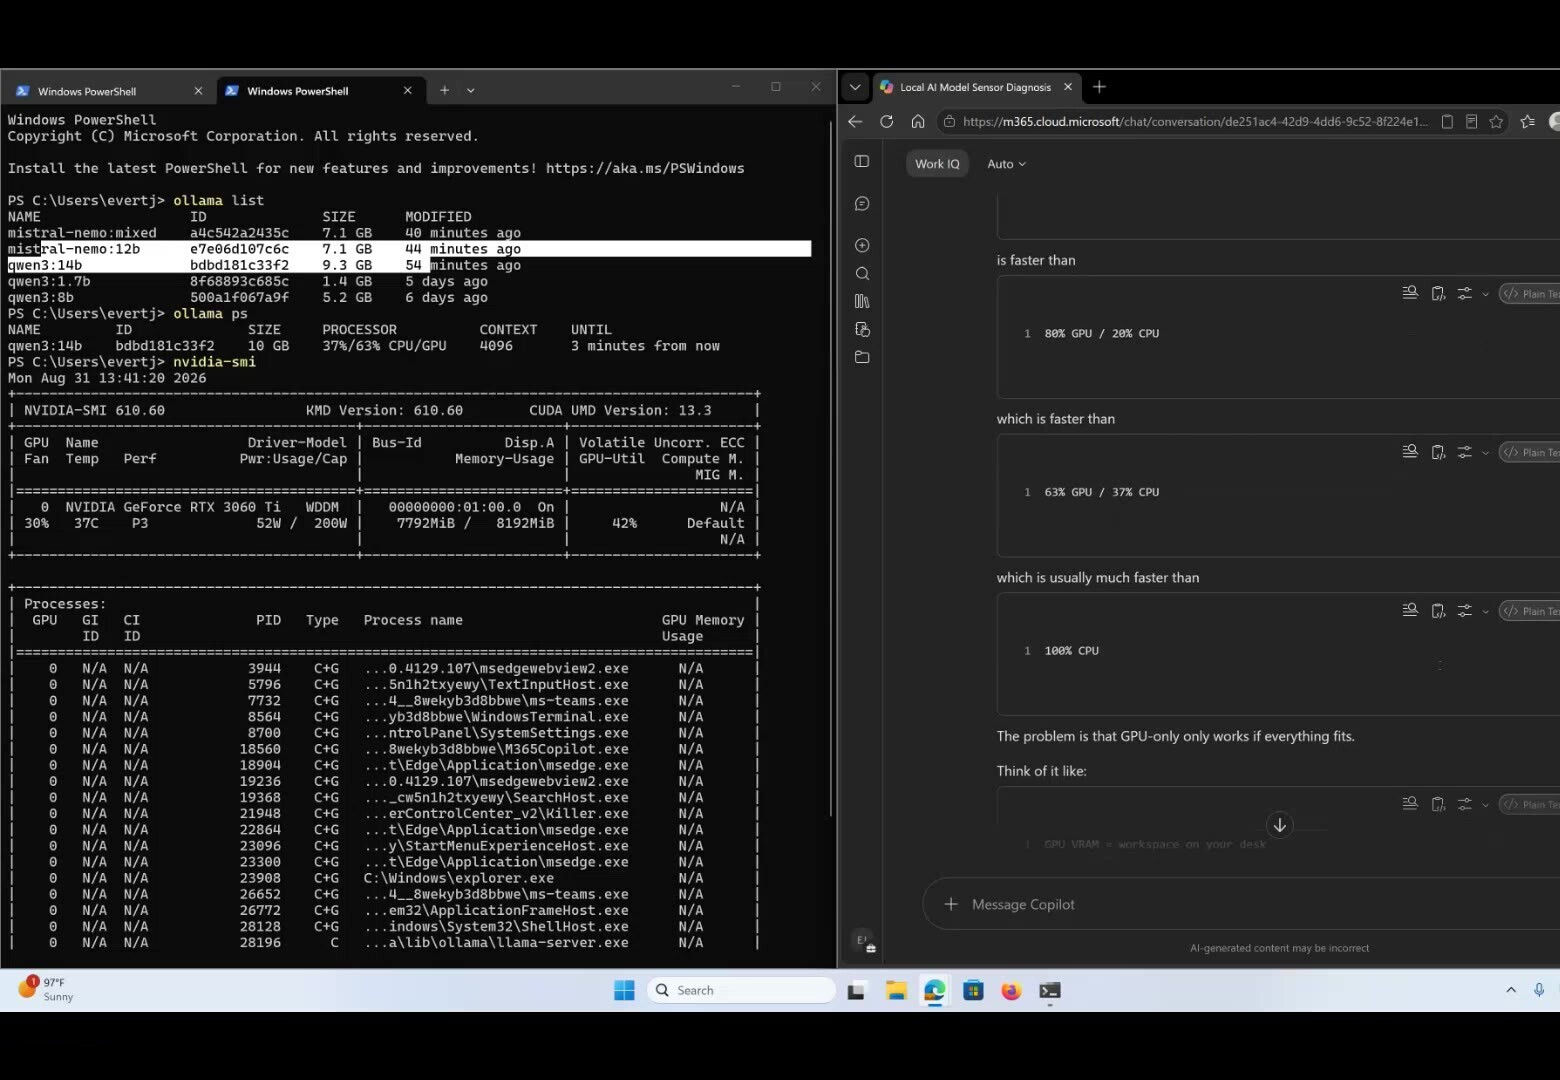
\includegraphics[width=.70\textwidth,height=.62\textheight,keepaspectratio]{split}
  \vfill\centering\small A split can make an oversized model run, but fit and speed are separate claims.
\end{frame}
\begin{recapframe}{Before next class}
  \begin{itemize}
    \item “Runs usefully” requires a bounded task and evidence.
    \item Hardware is a starting point; VRAM is a real boundary.
    \item A model's answer is a proposal until independently verified.
    \item Write World Bible v0.1 and leave its unknowns visible.
  \end{itemize}
\end{recapframe}
\end{document}
